\clearpage
\appendix
\section{Painéis completos de energia e construção}
\label{anexo:paineis}

\begin{figure}[!ht]
\centering
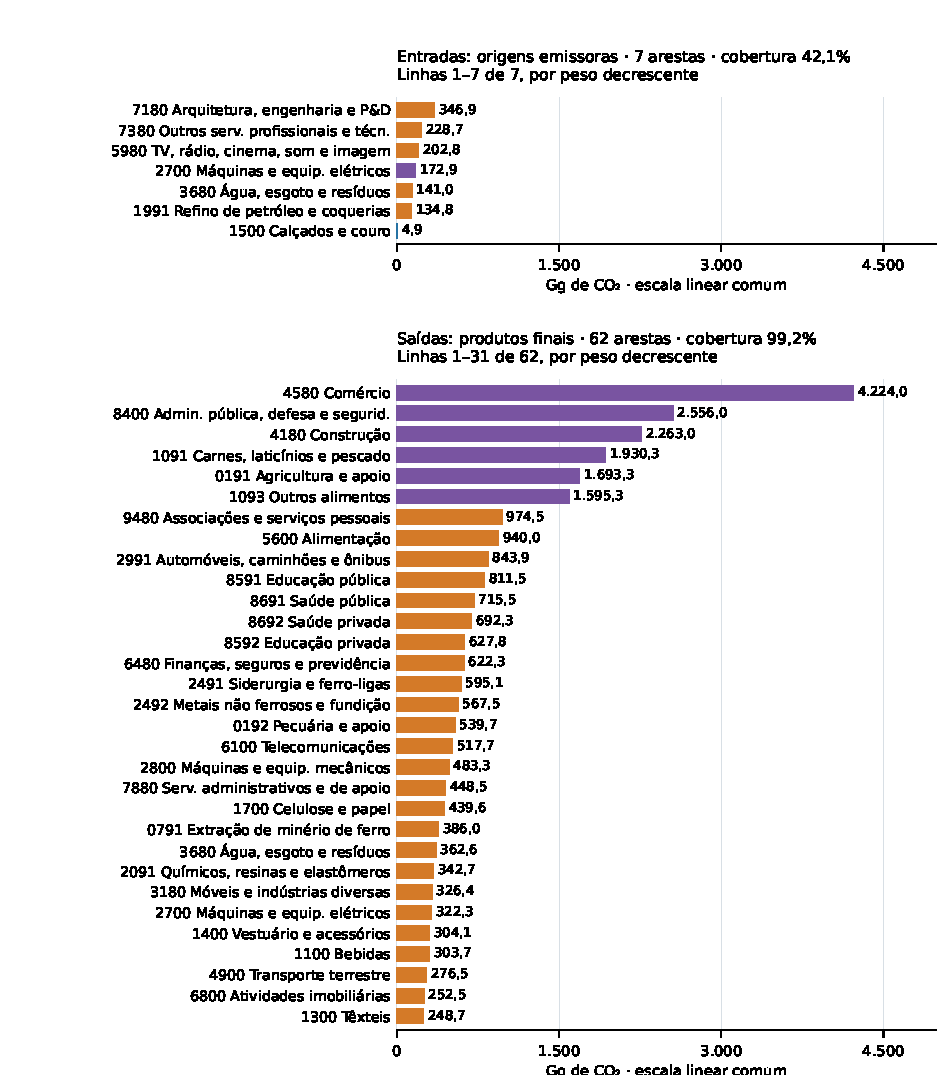
\includegraphics[width=\textwidth,height=0.78\textheight,keepaspectratio]{figuras/anexo_energia_1.pdf}
\caption{Energia (3500): todas as sete entradas e as saídas 1--31 de 62.}
\label{fig:anexo-energia}
\begin{minipage}{\textwidth}\footnotesize
Fonte: elaboração própria. Recortes de $\alpha=0{,}05$, com pesos originais em Gg de CO\textsubscript{2}, uma casa decimal e escala linear comum. A cobertura é o peso retido sobre a força da atividade e direção em $W$, sem diagonal: 42,1\% nas entradas e 99,2\% nas 62 saídas. As demais saídas aparecem na continuação, sem novo filtro. Azul: só saída na origem; laranja: só entrada no destino; roxo: ambos os testes.
\end{minipage}
\end{figure}
\clearpage
\begin{figure}[p]
\ContinuedFloat
\centering
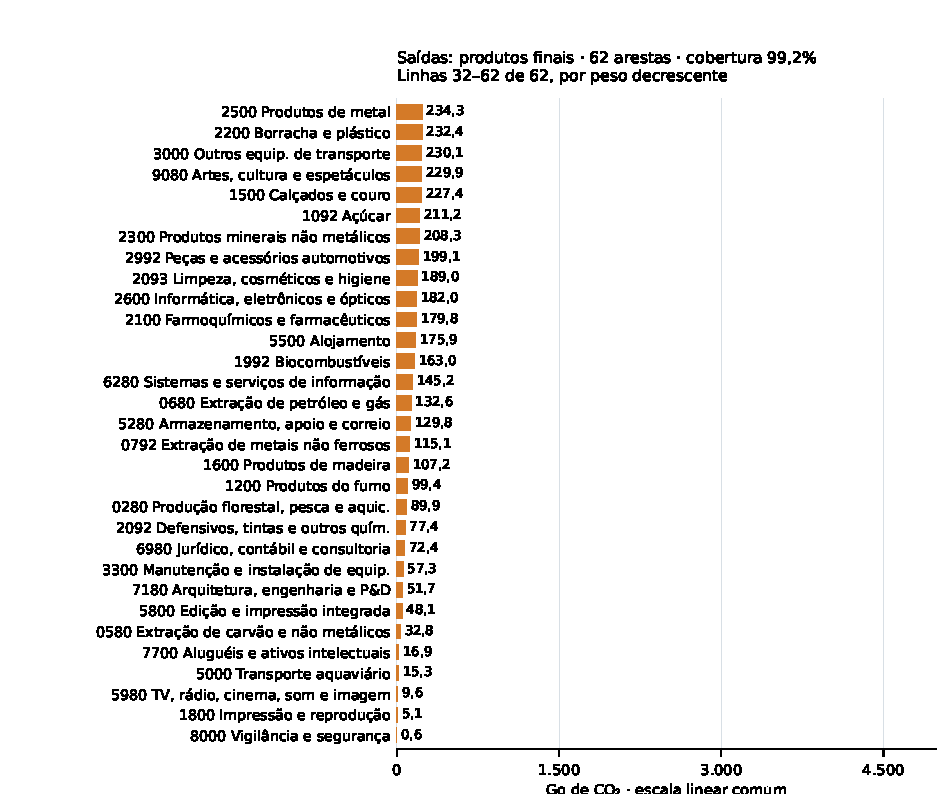
\includegraphics[width=\textwidth,height=0.85\textheight,keepaspectratio]{figuras/anexo_energia_2.pdf}
\caption{Energia (3500), continuação: saídas 32--62 de 62.}
\begin{minipage}{\textwidth}\footnotesize
Fonte: elaboração própria. Mesma seleção, ordem, escala e cores do painel anterior. A cobertura de 99,2\% se refere às 62 saídas, não apenas a esta página. Azul: só saída na origem; laranja: só entrada no destino; roxo: ambos os testes.
\end{minipage}
\end{figure}
\clearpage
\begin{figure}[p]
\centering
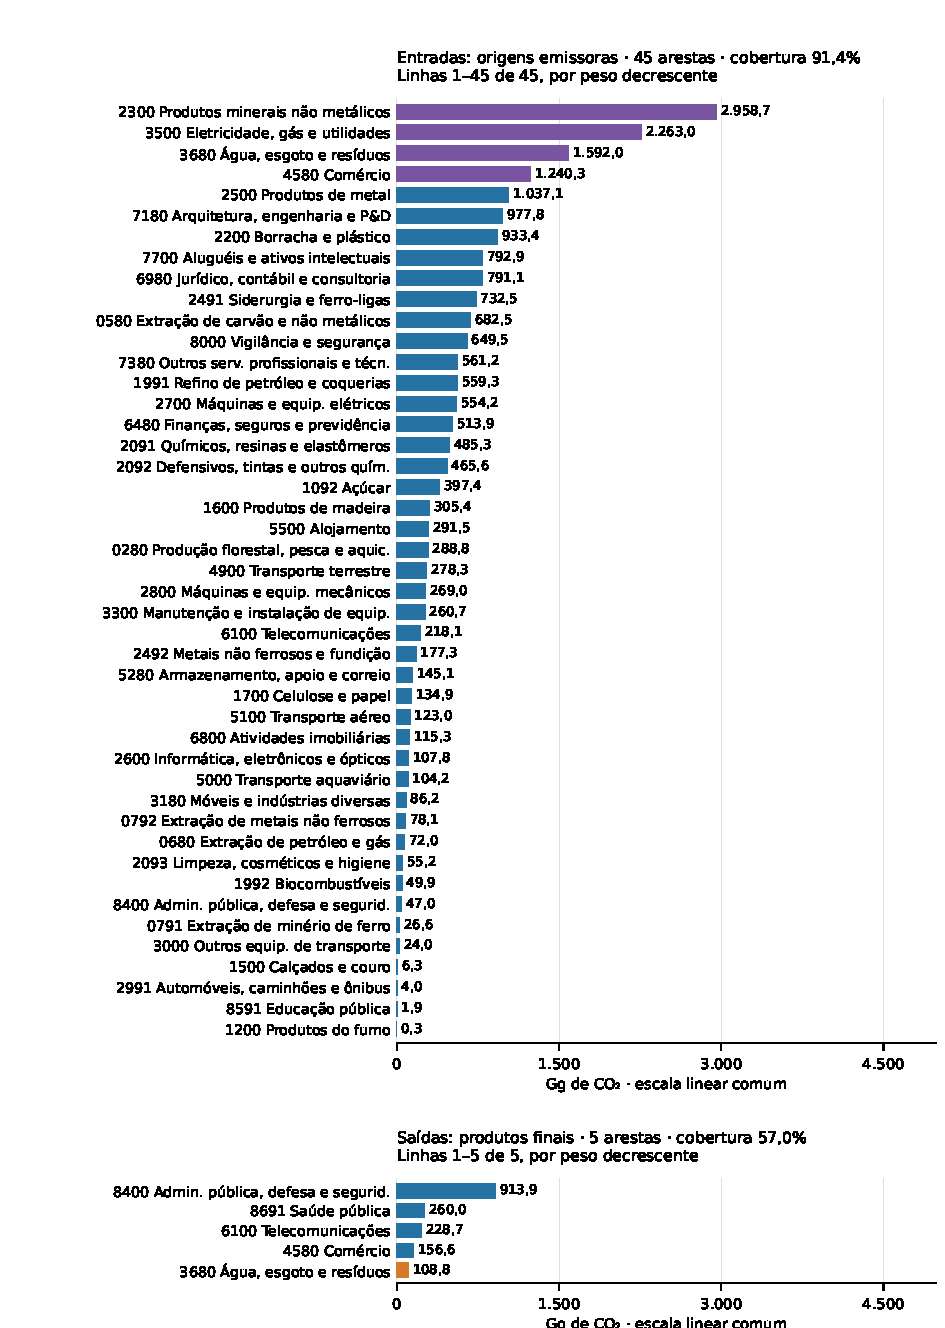
\includegraphics[width=\textwidth,height=0.85\textheight,keepaspectratio]{figuras/anexo_construcao.pdf}
\caption{Construção (4180): todas as 45 entradas e cinco saídas.}
\label{fig:anexo-construcao}
\begin{minipage}{\textwidth}\footnotesize
Fonte: elaboração própria. Coberturas de 91,4\% nas entradas e 57,0\% nas saídas. Mesma escala de pesos dos painéis de energia. Azul: só saída na origem; laranja: só entrada no destino; roxo: ambos os testes. Arestas compartilhadas não são duplicadas na rede.
\end{minipage}
\end{figure}
\clearpage

\section{Diagnósticos complementares da rede e da seleção}
\label{anexo:diagnosticos}

Na rede completa, os 66 perfis definidos têm medianas de 11,50 destinos efetivos e 13,93 origens efetivas, abaixo das 65 contrapartes existentes em cada direção. No backbone com $\alpha=0{,}05$, as medianas de cobertura são 59,32\% nas saídas e 55,69\% nas entradas.

A Tabela~\ref{tab:postos-complementares} detalha as mudanças de posição por grau em relação a $\alpha=0{,}05$. Os postos são calculados em ordem decrescente entre os 67 nós, com posto médio nos empates; reporta-se a mediana da mudança absoluta.

\begin{table}[htbp]
\centering
\caption{Mudança mediana de posição por grau em relação a $\alpha=0{,}05$.}
\label{tab:postos-complementares}
\begin{tabular}{@{}crr@{}}
\toprule
$\alpha$ & Grau de saída & Grau de entrada \\
\midrule
0,01 & 11 & 7 \\
0,10 & 4,5 & 4 \\
\bottomrule
\end{tabular}
\par\smallskip\begin{minipage}{\textwidth}\footnotesize
Fonte: elaboração própria. Valores em posições; as diferenças são calculadas a partir dos postos não arredondados, incluindo empates.
\end{minipage}
\end{table}

Dos 575 vínculos retidos em $\alpha=0{,}05$, 232 passam somente pelo teste de saída na origem, 265 somente pelo de entrada no destino e 78 pelos dois. Nenhum depende da convenção de grau um. A seleção por apenas uma extremidade mostra que uma relação pode destacar-se em um perfil sem ter a mesma importância relativa no outro.

Nos recortes da Tabela~\ref{tab:motivos-casos}, o backbone omite 57,9\% das entradas externas de energia e 43,0\% das saídas externas de construção. Esses complementos das coberturas evidenciam o volume omitido nas direções com menos ligações selecionadas.
